\chapter{\Chick{}: a core dependently-typed language and its repair
algorithm}~\label{chick}

This chapter will focus on the development and evaluation of a tool (named
\Chick{}\footnotemark{}) whose purpose is to help functional programmers
propagate changes, made to some of their definitions, to the rest of their code.

\footnotetext{All code for \Chick{} is publicly available at:
\url{https://github.com/Ptival/chick}}

Section~\ref{chick-background} gives background specific to this chapter.

Section~\ref{chick-design} describes the global design of the tool and its
components.

Section~\ref{chick-syntax} covers the syntax of the language over which \Chick{}
operates.

Section~\ref{chick-diffs} describes a family of data types that allow us to
perform repairs.

Section~\ref{chick-lookup} will present both usual lookup rules, and
\Chick{}-specific lookup rules, that are necessary to describe the repair
algorithm.

Section~\ref{chick-repair} describes all the components of the repair algorithm.

Section~\ref{chick-deriving} goes into more details into how some diff
operations needed by the repair algorithm can be automatically derived from
small descriptions of their reactions to certain changes in the data structure
they operate on.

Section~\ref{chick-guess}, finally, describes how we automatically infer diffs
from pairs of programs without requiring additional user input.

\section{Background}\label{chick-background}

Programs are rarely written once and for all: bugs may be found that must be
fixed, requirements may evolve in ways that require rewriting parts of a
program, and programs may be re-written in semantically-equivalent ways in order
to account for performance, resource-efficiency, or even simply stylistic
concerns.

The concept of \define{refactoring}, which was introduced as early as
in~\citet{wirfs1990surveying}, characterizes program transformations that
preserve the semantics of the program being manipulated.

% TODO FIXME

\section{Design}

We will now describe the syntax of our core language, \Chick{}, that will be the
target of our repair algorithm.  In sections~\ref{chick-design-syntax-terms}
and~\ref{chick-design-syntax-programs}, we will describe the syntax of its
terms, and programs, respectively.

\input{chick-design-syntax-terms}

\input{chick-design-syntax-programs}

\subsection{Describing program modifications with diffed data structures}\label{chick-design-diffs}

We define a family of data types that allows us to capture changes made to
programs from the language presented in
section~\ref{chick-design-syntax-programs}.  We will refer to these descriptions
of changes as \textit{diffs}.  We will usually denote a \textit{diff type}
$\delta_{\tau}$ if it corresponds to values of the diffed type $\tau$.  For
instance, the type $\delta_{\text{universe}}$ would capture how values of type
\coqinline{universe} may have been modified).

Importantly, note that we are not talking about values and types as they appear
in the user's program, but rather, about the internal values and types of the
meta-language.  For instance, if a user changes a \coqinline{bool} value in
their program from \coqinline{true} to \coqinline{false}, we will capture this
change using $\delta_{\text{term}}$, the diff type for $\synt{term}$; whereas
values of the diff type $\delta_{\text{bool}}$ would describe changes made to
boolean flags in the meta-language.

When the user makes a change to their program, we will attempt to guess the
structure of their changes, as a value of one of the program diff type
$\delta_{\text{program}}$.  To illustrate the kind of changes we are interested
in describing, let us go back to our motivating example in
Figure~\ref{listtovec}, where we can observe the following user-provided
modifications (dashed blue outline):

\begin{enumerate}

\item they renamed \coqinline{list} into \coqinline{vec},

\item added an index of type \coqinline{nat},

\item renamed constructor \coqinline{nil} into \coqinline{vnil},

\item instantiated the index for the first constructor with \coqinline{O},

\item renamed constructor \coqinline{cons} into \coqinline{vcons},

\item added a parameter \coqinline{n} of type \coqinline{nat} to the second
  constructor,

\item updated the recursive occurrence's name,

\item updated the recursive occurrence's index,

\item and instantiated the index for the second constructor with \coqinline{(S n)}.

\end{enumerate}

Intuitively, we want to capture changes like insertion, modifications,
deletions, and permutations, at all syntactic levels of the meta-language
(within terms, within inductive declarations).  We will use the same
descriptions to capture user-provided and repair-generated modifications.

Every diff type is accompanied by a patching function, which, given an element
of the diffed type and an element of the diff type produces, when successful, a
patched element.  This operation is partial for many diff types, because they
often capture modifications that only make sense for certain constructors of the
diffed type: for instance, a diff that says the head of a list has been modified
does not apply to the empty list.  We will overload the notation
$\MathPatches{x}{\delta_x}{x'}$ to indicate that $x'$ is the (optional) value
obtained when (successfully) patching $x$ according to the diff $\delta_x$,
using the relevant patching function for that diff type.  In all of our
notations, we use a black frame and a teal highlight to indicate that a value is
an output.

\subsection{Atomic diff}

There are many data types for which we will only capture changes at an atomic
granularity: either the value is the same in the new program, or it has been
replaced with a different, unrelated value.  For instance, a binder can either
have the same name, or have been renamed.  Similarly, the only possible change
to the recursive flag of a definition is to be atomically changed to a different
value.  The parameterized $\delta_{atomic}$ diff type captures such cases for a
given type $\tau$:

\begin{grammar}
<$\delta_{atomic}\ \tau$> ::= \ %trick LaTeX
\alt $\MathSame$                        \hfill (unchanged)
% \alt $\MathReplace{\langle\tau\rangle}$ \hfill (replaced)
\end{grammar}
%
with the following semantics:

\begin{mathpar}

  {
    \inferrule*
    [right=Identity]
    {  }
    {\MathPatches{x}{\MathSame}{x}}
  }

  {
    \inferrule*
    [right=Replace]
    {  }
    {\MathPatches{x}{\MathReplace{y}}{y}}
  }

\end{mathpar}

\subsection{List diff} \label{list-diff}

For lists, we provide a rich selection of diff operations.  The aim is not to
have a canonical representation, but rather to capture closely the intent of
the user modifications:

\begin{grammar}
<$\delta_{\text{list}} \ \tau \ \delta_{\tau}$> ::= \ %trick LaTeX
\alt \synt{$\delta_{\text{atomic}}\ \tau$} \hfill (atomic modification)
\alt \begin{tabular}{p{0.3cm} >{\centering}p{0.6cm} l}$\langle\tau\rangle$
       & $\MathIns{}{}$
       & \synt{$\delta_{list}\ \tau\ \delta_{\tau}$} \\\end{tabular} \hfill
     (insert a head)
\alt \begin{tabular}{p{0.3cm} >{\centering}p{0.6cm} l}$\langle\delta_\tau\rangle$
       & $\MathMod{}{}$
       & \synt{$\delta_{list}\ \tau\ \delta_{\tau}$} \\\end{tabular}
     \hfill (modify and keep the head)
%\alt \begin{tabular}{p{0.3cm} >{\centering}p{0.6cm} l}\quad & $\MathKeep{}$
%       & \synt{$\delta_{list}\ \tau\ \delta_{\tau}$} \\\end{tabular}
%     \hfill (keep the head)
\alt \begin{tabular}{p{0.3cm} >{\centering}p{0.6cm} l}\quad
       & $\MathDrop{}$
       & \synt{$\delta_{list}\ \tau\ \delta_{\tau}$} \\\end{tabular}
     \hfill (drop the head)
\alt \begin{tabular}{p{0.3cm} >{\centering}p{0.6cm} l}\quad
       & FIXME % $\MathPermute{p}{}$
       & \synt{$\delta_{\text{list}}\ \tau\ \delta_{\tau}$} \\\end{tabular}
     \hfill (permute according to a permutation $p$)
\end{grammar}
%
with the following semantics:

\begin{mathpar}
  {
    \inferrule*
    [right=Insert]
    {\MathPatches{l}{\delta_{l}}{l'}}
    {\MathPatches{l}{\MathIns{h}{\delta_{l}}}{(h :: l')}}
  }

  {
    \inferrule*
    [right=Modify]
    {\MathPatches{h}{\delta_{h}}{h'} \quad \MathPatches{t}{\delta_{t}}{t'}}
    {\MathPatches{(h :: t)}{\MathMod{\delta_{h}}{\delta_{t}}}{(h' :: t')}}
  }
\\
  % {
  %   \inferrule*
  %   [right=Keep]
  %   {\MathPatches{t}{\delta_{t}}{t'}}
  %   {\MathPatches{(h :: t)}{\MathKeep{\delta_{t}}}{(h :: t')}}
  % }
  {
    \inferrule*
    [right=Drop]
    {\MathPatches{t}{\delta_{t}}{t'}}
    {\MathPatches{(h :: t)}{\MathDrop{\delta_{t}}}{t'}}
  }

  {
    \inferrule*
    [right=Permute]
    {\MathPatches{(h_{p(1)} \Cons \ldots \Cons h_{p(|p|)} \Cons t)}{\delta}{l}}
    {\MathPatches{(h_1 \Cons \ldots \Cons h_{|p|} \Cons t)}{\MathPermute{p}{\delta}}{l}}
  }

\end{mathpar}

Note that we defined the semantics of $\MathModPiOp$ so that it both modifies
and keeps the head: the recursive occurrence in rule~\rulename{Modify},
$\delta_t$, therefore applies to the tail $t$ and not the whole list after the
head has been repaired.  On the other hand, the recursive occurrence in
rule~\rulename{Permute}, $\delta$, targets the entire list after the permutation
is performed, not solely the tail: this is necessary because we will want to
perform modifications of elements after having shuffled them around.

\subsection{Term diff}

The diffs for terms include atomic changes, as well as insertion, modification,
deletion, and permutation of most constructors.  We illustrate a couple of
these:

\begin{grammar}
<$\delta_{term}$> ::= \ %trick LaTeX
\alt \synt{$\delta_{atomic}\ t$} \hfill (atomic modification)
\alt \synt{$\delta_{term}$} $\oIns{ \$ }$ \synt{$\delta_{term}$} \hfill
(insert application)
\alt $\oIns{\lambda}$ \synt{v}, \synt{$\delta_{term}$} \hfill (insert value
abstraction)
\alt $\oIns{\Pi}$ (\synt{v} : \synt{$\delta_{term}$}),
\synt{$\delta_{term}$} \hfill (insert type abstraction)
\alt ... \hfill (other insertions)
\alt ... \hfill (removals/modifications/permutations)
\end{grammar}

\noindent Note that we use an infix dollar sign ($\$$) as a symbol for function
application in our diffs, even though we use an infix space for function
application in our terms, which is not ideal but should prevent confusion.  For
our purpose, we biased the diffs on binary operations in the least surprising
way: deleting an application keeps its left child, i.e. removes the function
call and keeps the function (see \rulename{\RmApp}), while deleting a
\coqinline{Pi} keeps its right child, i.e. removes the value being quantified
but keeps the return type (see \rulename{\RmPi}).  For insertion, we allow
maximal flexibility by passing the entire old term to all recursive occurrences:
for instance, the diff $(\MathInsApp{\MathSame}{\MathSame})$ turns any term $t$
into the self-application $(t\ t)$ (see \rulename{\InsApp}).  However, it is
often the case that only one recursive occurrence will use the original term,
while the other ones will replace it: for instance, the diff
$(\MathInsApp{\MathSame}{\MathReplace{x}})$ turns any term $t$ into the
application $(t\ x)$.

\begin{mathpar}
  {
    \inferrule*
    [right=\RmApp]
    {\MathPatches{f}{\delta}{f'}}
    {\MathPatches{f\ x}{\MathDropApp{\delta}}{f'}}
  }

  {
    \inferrule*
    [right=\RmPi]
    {\MathPatches{\tau_{2}}{\delta}{\tau_{2}'}}
    {\MathPatches{\MathPi{\tau_{1}}{x}{\tau_{2}}}{\MathDropPi{\delta}}{\tau_{2}'}}
  }

  {
    \inferrule*
    [right=\InsApp]
    {\MathPatches{t}{\delta_1}{t_1} \quad \MathPatches{t}{\delta_2}{t_2}}
    {\MathPatches{t}{\MathInsApp{\delta_1}{\delta_2}}{t_1\ t_2}}
  }

\end{mathpar}

\subsection{Other diff types}

We also need diffs for many other internal data types.  Diff types for tuples
are derived from diff types of their constituents in a straightforward way.
Inductive data type definitions, as well as constructor definitions, behave
essentially like a tuple of all their arguments, so their diff type is derived
accordingly.


\input{chick-design-repair}

\section{Syntax of \Chick{}}\label{chick-syntax}

This section will cover the syntax of \Chick{}.
Section~\ref{chick-syntax-terms} describes the syntax of the terms of the
language, a language similar to \Coq{}'s \Gallina{}.
Section~\ref{chick-syntax-programs} describes the syntax of the host language, a
language similar to \Coq{}'s \Vernacular{}, within which functions and data
types can be defined.

\subsection{Syntax of \Chick{} terms}\label{chick-syntax-terms}

\Chick{} is designed as a small functional programming language upon which the
repair algorithm will operate.  The aim was to represent a language such as
\Gallina{}, and as such, \Chick{} is a dependently-typed lambda calculus, with
inductive constructions.  The abstract syntax of \Chick{} terms is given in the
following grammar:

\begin{grammar}%
<term> ::= \ %trick LaTeX
\alt <term> \coqinline{:} <term>                         \hfill (type annotation)
\alt <term> <term>                                       \hfill (function application)
\alt \coqinline{_}                                       \hfill (hole)
\alt \coqinline{λ} <binder> \coqinline{,} <term>         \hfill (value abstraction)
\alt \coqinline{match} <term> \coqinline{with}
$\overline{ \synt{pattern} }$ \coqinline{end}            \hfill (pattern matching)
\alt \coqinline{Π(} <binder> \coqinline{:} <term>
\coqinline{) →} <term>                                   \hfill (type abstraction)
\alt <universe>                                          \hfill (universes)
\alt <var>                                               \hfill (variable)

<universe> ::= \coqinline{Prop} | \coqinline{Set} | \coqinline{Type}

<binder> ::= \ % trick LaTeX
\alt <var> \hfill (named)
\alt _     \hfill (anonymous)

<pattern> ::= ($\overline{ \synt{binder} }$, <term>)
\end{grammar}

The \emph{function application}, \emph{value abstraction}, \emph{type
abstraction}, and \emph{variable} constructs, are standard constructs of a
dependently-typed lambda calculus.

The \emph{type annotation} construct lets us ascribe a type to a given term.
The \emph{hole} construct can take the place of a term anywhere: it stands for a
missing value that should be filled by the programmer.  Together, these two
constructs let us have \define{typed holes}, that is, placeholder values whose
type is known.  This proves invaluable throughout the repair algorithm, as we
will see, since there are situations where the algorithm must come up with
arbitrary values, knowing only the type they should bear.  In the absence of
synthesis techniques to generate such values, the algorithm can safely insert a
typed hole, leaving to the programmer the task of figuring out the proper value.

Finally, the \emph{pattern matching} construct is found in languages with
algebraic data types, and lets us dispatch code based on the shape of some such
data type.  The attentive reader may notice that our pattern language is
somewhat limited.  We do not cover nested patterns, or other advanced pattern
features.

We use the same universe names as found in \Gallina{}, though we do not yet
support its cumulative universe hierarchy syntactically.  This does \emph{not}
mean that \Chick{} cannot repair \Gallina{} programs that use the universe
hierarchy, but rather, that it cannot syntactically represent universe levels.
Instead, \Chick{} is oblivious to universe levels, so it will repair programs
regardless of their universe level.  The downside is that, because it cannot
represent universe levels explicitly, it might break programs that require them.
Bare support for universe levels can be added almost for free, since the repair
algorithm could simply carry them along and attempt no repair.  A universe-aware
repair algorithm would require further investigation.

\paragraph{About underscores} While we use the underscore symbol ($\_$) to
represent both a hole term and an anonymous binder, the two concepts can never
appear in the same program location, and therefore, there can be no confusion:
in a term context, the symbol represents a hole, while in a binding context, it
represents an anonymous binder.


\subsection{Syntax of \Chick{} programs}\label{chick-syntax-programs}

Our programs are defined as sequences of commands in the following vernacular
(to borrow Coq's parlance):

\begin{grammar}
<program> ::= $\overline{ \synt{vernacular} }$

<vernacular> ::= \ %trick LaTeX
\alt \coqinline{Definition}(\{ kind : <definition-kind> , name : <var>, type : <term>, body : <term> \})
\alt \coqinline{Inductive}(<inductive>)

<definition-kind> ::= \coqinline{Definition} | \coqinline{Fixpoint}
\end{grammar}

Our \define{definition kinds} follow \Coq{}'s \Vernacular{} conventions: a
\coqinline{Definition} is \emph{never} recursive, while a \coqinline{Fixpoint}
is \emph{allowed} to be recursive.  Declarations are ordered, and may only
depend on previous declarations.  This will ease the task of our repair
algorithm, since dependencies are syntactically ordered.  In a language where
declarations are allowed to depend on other declarations backward \emph{and}
forward, we would want to repair programs according to the dependency tree
rather than the syntactic order of declarations.

Inductive definitions are not mutual, and follow the following syntax:

\noindent
\begin{grammar}
<inductive> ::= \coqinline{Inductive}(\{\\
name : \synt{var},\\
parameters : $\overline{ ( \synt{var} , \synt{term} ) }$,\\
indices : $\overline{ ( \synt{binder} , \synt{term} ) }$,\\
universe : \synt{universe},\\
constructors : $\overline{ \synt{constructor} }$\\
\})

<constructor> ::= \coqinline{Constructor}(\{\\
name : \synt{var},\\
parameters : $\overline{ ( \synt{binder}, \synt{term} ) }$,\\
indices : $\overline{ \synt{term} }$\\
\})
\end{grammar}

For a presentation of inductive data type declarations, we refer the reader
to~\mycite{coquand1990inductively} for an academic description, or
to~\mycite{pierce2010software} for some educational material.  We will briefly
recall the difference between \define{inductive parameters}, \define{inductive
indices}, \define{constructor parameters}, and \define{constructor indices}.

\define{Inductive parameters} indicate that a type is generic in some input
type.  Most often, this type parameter will be a type that the constructors may
contain instances of, or operate on values of.  For instance, many containers
will have a carrier type for the type of values they may contain.  The choice of
type to be contained does \emph{not} restrict the shapes that the container may
take: we say that it behaves \emph{parametrically}.  For instance, the type of
list of boolean values, \coqinline{list bool}, and the type of list of natural
number values, \coqinline{list nat}, contain the same ``shapes'':
\coqinline{[]}, \coqinline{_ ∷ []}, \coqinline{_ ∷ _ ∷ []}, etc.  The choice of
the type parameter only tells us what values we are allowed to put in those
holes, but does not dictate which of those shapes we may or may not instantiate.

On the other hand, \define{inductive indices} can affect what inhabitants we may
find in an inductive type.  Instead of being called an inductive type, one that
is indexed is often instead called an \define{inductive family of types}, or
\define{inductive type family}, to capture the idea that the choice of index has
an effect on what inhabitants may exist.  Knowing the index of an inductive
value gives us information about what shape it may have.  For instance, we could
build a type of lists indexed by whether their length is odd or even as:%
%
\footnote{\Coq{} syntax does not let us define constructors that look like
operators, but we do it here to keep the code clear and concise.}%
%
\textsuperscript{,}%
%
\footnote{In constructor \coqinline{(∷)}, we use curly braces \coqinline{p} to
mark the constructor parameter as implicit, indicating it can be implicitly
inserted unambiguously by Coq when the next constructor parameter,
\coqinline{t}, is supplied.}

\begin{minted}{coq}
Inductive parity : Type :=
| Even : parity
| Odd  : parity
.

Definition next_parity (p : parity) : parity :=
  match p with
  | Even => Odd
  | Odd  => Even
  end.

Inductive parity_list (T : Type) : parity → Type :=
| []  : parity_list T Even
| (∷) : ∀ (h : T) {p : parity} (t : parity_list T p) →
        parity_list T (next_parity p)
.
\end{minted}

Now, if we consider the type family \coqinline{parity_list T p} as a whole, for
a given choice of carrier type \coqinline{T}, the possible shapes of values are
still the same as for \coqinline{list}: \coqinline{[]}, \coqinline{_ ∷ []},
\coqinline{_ ∷ _ ∷ []}, etc.  However, for a given choice of \coqinline{p}, the
valid shapes become restricted by construction.  The type \coqinline{parity_list
T Even} only contains shapes \coqinline{[]}, \coqinline{_ ∷ _ ∷ []},
\coqinline{_ ∷ _ ∷ _ ∷ _ ∷ []}, etc.  Dually, the type \coqinline{parity_list T
Odd} only contains shapes \coqinline{_ ∷ []}, \coqinline{_ ∷ _ ∷ _ ∷ []}, etc.

In general, different families may have entirely disjoint shapes, as presented
here, or partially-overlapping shapes (for instance, the type family of finite
sets), or even all the same shapes (in which case, the index might be used as a
type-level marker for some information, a technique often called \coqinline{phantom
type} in statically-typed languages).

\define{Constructor parameters} are just arguments that are passed to a given
constructor.  They are completely independent for each constructor, and are
simply used to store data relevant to the given constructor.  For instance, in
our \coqinline{parity_list} example, \coqinline{h}, \coqinline{p}, and
\coqinline{t} are three constructor parameters for constructor \coqinline{(∷)}.

The return type of a constructor must indicate in what family is exists.  To do
so, it must provide values for the inductive indices.  We call those values the
\define{constructor indices}.  For instance, in our \coqinline{parity_list}
example, the inductive index of type \coqinline{parity} is instantiated with
value \coqinline{(next_parity p)} in the \coqinline{(∷)} constructor.  Note that
it is possible to have indices be computed values, as is the case here.

Finally, let us discuss scope for those constructs.

\begin{itemize}

\item Following \Coq{}'s convention, inductive parameters \emph{must} be named.
They are naturally in scope for the whole definition of the inductive type.

\item Inductive indices \emph{may} be anonymous, or named, and they form a
telescope (as described in Section~\ref{dependenty-types}).  They are \emph{not}
scoped over the rest of the definition.  Therefore, the only purpose for named
indices is to create dependent indices.

\item Constructor parameters \emph{may} be anonymous, or named.  They also form
a telescope all the way to the constructor's return type, such that both
subsequent parameters, as well as the constructor's indices, may refer to them.

\item Constructor indices \emph{must} be passed as explicit arguments to the
return type, and as such, there is no binding involved.

\end{itemize}


\subsection{Describing program modifications with
diffs}\label{chick-diffs}

We define a family of data types that allows us to describe changes made to
programs from the language presented in Section~\ref{chick-syntax-programs}.  We
will refer to these descriptions of changes as \textit{diffs}.  We will usually
denote a \textit{diff type} $\delta_{\tau}$ if it corresponds to values of the
diffed type $\tau$.  Informally, one can think of the type $\delta_{\tau}$ as a
descriptor for how some value $v_{1}$ of type $\tau$ can be transformed into
another value $v_{2}$.

It is important to clarify how we intend to use those diff types.  We will want
to describe changes made to the data types in the abstract syntax tree of the
user's program.  An example will help us avoid some misconception: consider the
user program and its modification in Figure~\ref{bool-modification}.  While,
from the program point of view, a value of type \coqinline{bool} was modified
from the value \coqinline{True} to the value \coqinline{False}, we will
\emph{not} use the type $\delta_{\coqinline{bool}}$ to describe this change!
From the point of view of the abstract syntax tree, a value of type
\coqinline{term} has changed from the original value \coqinline{Var "True"} to
the value \coqinline{Var "False"}, which we will capture using the diff type
$\delta_{\coqinline{term}}$.

To be precise, we will have to describe how a \coqinline{Definition} has
changed, and describe how its name has remained \coqinline{a}, its type has
remained \coqinline{bool}, but its definition has changed.  This will be
described as a value of type $\delta_{\coqinline{vernac}}$, containing a diff
for each of those three components that may change, including the one of diff
type $\delta_{\coqinline{term}}$.

\begin{figure*}[!htp]

  \noindent%
  \begin{minipage}[t]{0.50\textwidth}
    \begin{minted}[linenos=false]{coq}
Inductive bool : Set :=
| True  : bool
| False : bool.

Definition a : bool := True.
\end{minted}
\end{minipage}%
\begin{minipage}[t]{0.50\textwidth}
  \begin{minted}[escapeinside=@@,linenos=false]{coq}
Inductive bool : Set :=
| True  : bool
| False : bool.

Definition a : bool := @\modified{False}@.
\end{minted}
\end{minipage}

\caption{A simple program and its modification.}

\label{bool-modification}

\end{figure*}

When the user makes a change to their program, we will attempt to guess the
structure of their changes, as a value of one of the program diff type
$\delta_{\coqinline{program}}$.  To illustrate the kind of changes we are
interested in describing, let us look back at our motivating example in
Figure~\ref{listtovec}, where we can observe the following partial attempts at
refactoring:

\begin{enumerate}

\item they renamed \coqinline{list} into \coqinline{vec},

\item added an index of type \coqinline{nat},

\item renamed constructor \coqinline{nil} into \coqinline{vnil},

\item instantiated the index for the first constructor with \coqinline{O},

\item renamed constructor \coqinline{cons} into \coqinline{vcons},

\item added a parameter \coqinline{n} of type \coqinline{nat} to the second
  constructor,

\item updated the recursive occurrence's name,

\item updated the recursive occurrence's index,

\item and instantiated the index for the second constructor with \coqinline{(S n)}.

\end{enumerate}

Intuitively, we want to capture changes like insertion, modifications,
deletions, and permutations, at all syntactic levels of the meta-language
(within terms, within inductive declarations).  We will use the same
descriptions to capture user-provided and repair-generated modifications.

Every diff type is accompanied by a patching function, which, given an element
of the diffed type and an element of the diff type produces, when successful, a
patched element.  This operation is partial for many diff types, because they
often capture modifications that only make sense for certain constructors of the
diffed type: for instance, a diff that says the head of a list has been modified
does not apply to the empty list.  We will overload the notation
$\MathPatches{x}{\delta_x}{x'}$ to indicate that $x'$ is the (optional) value
obtained when (successfully) patching $x$ according to the diff $\delta_x$,
using the relevant patching function for that diff type.  In all of our
notations, we use a black frame and a teal highlight to indicate that a value is
an output.

\subsection{Atomic diff}

There are many data types for which we will only capture changes at an atomic
granularity: either the value is the same in the new program, or it has been
replaced with a different, unrelated value.  For instance, a binder can either
have the same name, or have been renamed.  Similarly, the only possible change
to the recursive flag of a definition is to be atomically changed to a different
value.  The parameterized $\delta_{atomic}$ diff type captures such cases for a
given type $\tau$:

\begin{grammar}
<$\delta_{atomic}\ \tau$> ::= \ %trick LaTeX
\alt $\MathSame$                        \hfill (unchanged)
% \alt $\MathReplace{\langle\tau\rangle}$ \hfill (replaced)
\end{grammar}
%
with the following semantics:

\begin{mathpar}

  {
    \inferrule*
    [right=Identity]
    {  }
    {\MathPatches{x}{\MathSame}{x}}
  }

  {
    \inferrule*
    [right=Replace]
    {  }
    {\MathPatches{x}{\MathReplace{y}}{y}}
  }

\end{mathpar}

\subsection{List diff} \label{list-diff}

\subsubsection{Syntax}

For lists, we provide a rich selection of diff operations.  The aim is not to
have a canonical representation, but rather to capture closely the intent of
the user modifications:

\begin{grammar}
<$\delta_{\text{list}} \ \tau \ \delta_{\tau}$> ::= \ %trick LaTeX
\alt \synt{$\delta_{\text{atomic}}\ \tau$} \hfill (atomic modification)
\alt \begin{tabular}{p{0.7cm} >{\centering}p{0.7cm} l}$\langle\tau\rangle$
       & $\MathIns{}{}$
       & \synt{$\delta_{list}\ \tau\ \delta_{\tau}$} \\\end{tabular} \hfill
     (insert a head)
\alt \begin{tabular}{p{0.7cm} >{\centering}p{0.7cm} l}$\langle\delta_\tau\rangle$
       & $\MathMod{}{}$
       & \synt{$\delta_{list}\ \tau\ \delta_{\tau}$} \\\end{tabular}
     \hfill (modify and keep the head)
%\alt \begin{tabular}{p{0.3cm} >{\centering}p{0.6cm} l}\quad & $\MathKeep{}$
%       & \synt{$\delta_{list}\ \tau\ \delta_{\tau}$} \\\end{tabular}
%     \hfill (keep the head)
\alt \begin{tabular}{p{0.7cm} >{\centering}p{0.7cm} l}\quad
       & $\MathDrop{}$
       & \synt{$\delta_{list}\ \tau\ \delta_{\tau}$} \\\end{tabular}
     \hfill (drop the head)
\alt \begin{tabular}{p{0.7cm} >{\centering}p{0.7cm} l}\quad
       & $\MathPermute{p}{}$
       & \synt{$\delta_{\text{list}}\ \tau\ \delta_{\tau}$} \\\end{tabular}
     \hfill (permute according to a permutation $p$)
\end{grammar}
%
with the following semantics:

\begin{mathpar}
  {
    \inferrule*
    [right=Insert]
    {\MathPatches{l}{\delta_{l}}{l'}}
    {\MathPatches{l}{\MathIns{h}{\delta_{l}}}{(h :: l')}}
  }

  {
    \inferrule*
    [right=Modify]
    {\MathPatches{h}{\delta_{h}}{h'} \quad \MathPatches{t}{\delta_{t}}{t'}}
    {\MathPatches{(h :: t)}{\MathMod{\delta_{h}}{\delta_{t}}}{(h' :: t')}}
  }
\\
  % {
  %   \inferrule*
  %   [right=Keep]
  %   {\MathPatches{t}{\delta_{t}}{t'}}
  %   {\MathPatches{(h :: t)}{\MathKeep{\delta_{t}}}{(h :: t')}}
  % }
  {
    \inferrule*
    [right=Drop]
    {\MathPatches{t}{\delta_{t}}{t'}}
    {\MathPatches{(h :: t)}{\MathDrop{\delta_{t}}}{t'}}
  }

  {
    \inferrule*
    [right=Permute]
    {\MathPatches{(h_{p(1)} \Cons \ldots \Cons h_{p(|p|)} \Cons t)}{\delta}{l}}
    {\MathPatches{(h_1 \Cons \ldots \Cons h_{|p|} \Cons t)}{\MathPermute{p}{\delta}}{l}}
  }

\end{mathpar}

Note that we defined the semantics of $\MathModPiOp$ so that it both modifies
and keeps the head: the recursive occurrence in rule~\rulename{Modify},
$\delta_t$, therefore applies to the tail $t$ and not the whole list after the
head has been repaired.  On the other hand, the recursive occurrence in
rule~\rulename{Permute}, $\delta$, targets the entire list after the permutation
is performed, not solely the tail: this is necessary because we will want to
perform modifications of elements after having shuffled them around.

\subsection{Term diff}

The diffs for terms include atomic changes, as well as insertion, modification,
deletion, and permutation of most constructors.  We illustrate a couple of
these:

\begin{grammar}
<$\delta_{term}$> ::= \ %trick LaTeX
\alt \synt{$\delta_{atomic}\ t$} \hfill (atomic modification)
\alt \synt{$\delta_{term}$} $\oIns{ \$ }$ \synt{$\delta_{term}$} \hfill
(insert application)
\alt $\oIns{\lambda}$ \synt{v}, \synt{$\delta_{term}$} \hfill (insert value
abstraction)
\alt $\oIns{\Pi}$ (\synt{v} : \synt{$\delta_{term}$}),
\synt{$\delta_{term}$} \hfill (insert type abstraction)
\alt ... \hfill (other insertions)
\alt ... \hfill (removals/modifications/permutations)
\end{grammar}

\noindent Note that we use an infix dollar sign ($\$$) as a symbol for function
application in our diffs, even though we use an infix space for function
application in our terms, which is not ideal but should prevent confusion.  For
our purpose, we biased the diffs on binary operations in the least surprising
way: deleting a function application keeps its left child, i.e. removes the
function call and keeps the function (see rule~\rulename{\RmApp}), while
deleting a \coqinline{Pi} keeps its right child, i.e. removes the value being
quantified but keeps the return type (see rule~\rulename{\RmPi}).  For
insertion, we allow maximal flexibility by passing the entire old term to all
recursive occurrences: for instance, the diff
$(\MathInsApp{\MathSame}{\MathSame})$ turns any term $t$ into the
self-application $(t\ t)$ (see rule~\rulename{\InsApp}).  However, it is often
the case that only one recursive occurrence will use the original term, while
the other ones will replace it: for instance, the diff
$(\MathInsApp{\MathSame}{\MathReplace{x}})$ turns any term $t$ into the
application $(t\ x)$.

\begin{mathpar}
  {
    \inferrule*
    [right=\RmApp]
    {\MathPatches{f}{\delta}{f'}}
    {\MathPatches{f\ x}{\MathDropApp{\delta}}{f'}}
  }

  {
    \inferrule*
    [right=\RmPi]
    {\MathPatches{\tau_{2}}{\delta}{\tau_{2}'}}
    {\MathPatches{\MathPi{\tau_{1}}{x}{\tau_{2}}}{\MathDropPi{\delta}}{\tau_{2}'}}
  }

\\

  {
    \inferrule*
    [right=\InsApp]
    {\MathPatches{t}{\delta_1}{t_1} \quad \MathPatches{t}{\delta_2}{t_2}}
    {\MathPatches{t}{\MathInsApp{\delta_1}{\delta_2}}{t_1\ t_2}}
  }

\end{mathpar}

\subsection{Other diff types}

We also need diffs for many other internal data types.  Diff types for tuples
are derived from diff types of their constituents in a straightforward way.
Inductive data type definitions, as well as constructor definitions, behave
essentially like a tuple of all their arguments, so their diff type is derived
accordingly.

\section{Lookup rules for diffs}

\documentclass[preview]{standalone}

\usepackage{fontspec}
\usepackage{gfsdidot}          % makes math stuff look neat, but also overrides text stuff
\setmainfont{TeX Gyre Pagella} % forces back text stuff to look neat too
\setmonofont{DejaVuSansMono}   % monospace stuff should look neat too

\usepackage[dvipsnames]{xcolor} % must be loaded prior to tikz, pgfplots, etc.
\let\iint\relax
\let\iiint\relax
\let\iiiint\relax
\let\idotsint\relax
\usepackage{amsmath} % loaded by mathtools?
\usepackage{amssymb}
\usepackage[english]{babel}
\usepackage{booktabs}
\usepackage{calc}
\usepackage{caption}
\usepackage{color}
\usepackage{DejaVuSansMono}
\usepackage{dsfont}
\let\textlozenge\relax
\usepackage[inline]{enumitem}
\usepackage{environ}
\usepackage{etoolbox}
\usepackage{fontawesome}
\usepackage{forest}
\usepackage{graphicx}
\usepackage{longtable}
\usepackage{ltablex} \keepXColumns % Made me sad for appendix tables, where was it used?
\usepackage{makecell}
\usepackage{mathpartir}
%\usepackage{mathtools} % \coloneqq
\usepackage{mdframed}
\usepackage{minted}
\usepackage{multicol}
\usepackage[parfill]{parskip}
\usepackage{pgfplots}
\usepackage{pifont} % \ding
\usepackage{soul}
\usepackage{syntax}
\usepackage{tabularx}
\usepackage[skins,theorems]{tcolorbox}
\usepackage{tikz}
\usepackage{tikzpeople}
\usepackage{tikz-qtree}
\usepackage{xpatch}
\usepackage[breaklinks=true,pdfborder={0 0 0}]{hyperref}

% gfsdidot makes ∀ and ∃ super ugly, this reverts them to something fine
\DeclareSymbolFont{CMsymbols}{OMS}{cmsy}{b}{n}
\SetSymbolFont{CMsymbols}{bold}{OMS}{cmsy}{ub}{n}
\DeclareMathSymbol{\forall}{\mathord}{CMsymbols}{"38}
\DeclareMathSymbol{\exists}{\mathord}{CMsymbols}{"39}

\definecolor{monokaibg}{HTML}{272822}
\definecolor{color01}{HTML}{E6194B}
\definecolor{color02}{HTML}{3CB44B}
\definecolor{color03}{HTML}{FFE119}
\definecolor{color04}{HTML}{4363D8}
\definecolor{color05}{HTML}{F58231}
\definecolor{color06}{HTML}{911EB4}
\definecolor{color07}{HTML}{46F0F0}
\definecolor{color08}{HTML}{F032E6}
\definecolor{color09}{HTML}{BCF60C}
\definecolor{color10}{HTML}{FABEBE}
\definecolor{color11}{HTML}{008080}
\definecolor{color12}{HTML}{E6BEFF}
\definecolor{color13}{HTML}{9A6324}
\definecolor{color14}{HTML}{FFFAC8}
\definecolor{color15}{HTML}{800000}
\definecolor{color16}{HTML}{AAFFC3}
\definecolor{color17}{HTML}{808000}
\definecolor{color18}{HTML}{FFD8B1}
\definecolor{color19}{HTML}{000075}
\definecolor{color20}{HTML}{808080}
\definecolor{color21}{HTML}{FFFFFF}
\definecolor{color22}{HTML}{000000}

\def\mathunderline#1#2{\color{#1}\underline{{\color{black}#2}}\color{black}}

\forestset{
  default preamble={
    for tree={
      align=center,
      draw=black,
      edge={
        ultra thick,
      },
      edge path={
        \noexpand\path[\forestoption{edge}]
        (!u.parent anchor)
        -- +(0,-10pt)
        -| (.child anchor)
        \forestoption{edge label};
      },
      font=\bfseries,
      % inner sep=10pt,
      l sep=30pt,
      % line width=2pt,
      minimum height=20pt,
      minimum width=30pt,
      parent anchor=south,
      rectangle,
      ultra thick,
    }
  }
}

\newcolumntype{Y}{>{\centering\arraybackslash}X}

% defines safecoqinline, a command like coqinline but works in tabular
% environments
\makeatletter
\def\safecoqinline#1{%
\ifx\@footnotetext\TX@trial@ftn
\detokenize{#1}%
\else
\coqinline{#1}%
\fi}
\makeatother

\captionsetup{
  justification=centering,
}

\usetikzlibrary{arrows, calc, fit, positioning, shapes, tikzmark}

\tikzset{
bicolor/.style 2 args={
  dashed,dash pattern=on 4pt off 4pt,#1,
  postaction={draw,dashed,dash pattern=on 4pt off 4pt,#2,dash phase=4pt}
  },
}

\tikzstyle{Matching}=[
black,
dashed,
line width=3pt,
]

\tikzstyle{RoundedDottedPath}=[
densely dotted,
color05,
line width=3pt,
rounded corners=10pt,
]

\tikzstyle{RoundedRectangle}=[
dashed,
draw,
line width=3pt,
rounded corners=10pt,
]

\tikzstyle{NodeLabel}=[
black,
circle,
draw,
fill=white,
font=\bfseries,
inner sep=1pt,
ultra thick,
]

\graphicspath{ {./images/} }

% Fix a mdframed bug where skipbelow is ignored
% \makeatletter
% \xpatchcmd{\endmdframed}
%   {\aftergroup\endmdf@trivlist\color@endgroup}
%   {\endmdf@trivlist\color@endgroup\@doendpe}
%   {}{}
% \makeatother

% \surroundwithmdframed[
% backgroundcolor=monokaibg,
% linecolor=white,
% skipabove=1em,
% skipbelow=1em,
% leftmargin=10pt,
% innertopmargin=1pt,
% innerbottommargin=0pt
% ]{minted}

\setminted{
  % DO NOT use bgcolor, use mdframed instead
  % bgcolor=monokaibg,
  linenos=true,
  style=lovelace,
  breaklines=true,
  encoding=utf8,
  fontsize=\large,
  baselinestretch=1,
}

% need bgcolor for the display to be nice in rules
\newmintinline{coq}{bgcolor=white}

\makeatletter
\pgfdeclareshape{document}{
\inheritsavedanchors[from=rectangle] % this is nearly a rectangle
\inheritanchorborder[from=rectangle]
\inheritanchor[from=rectangle]{center}
\inheritanchor[from=rectangle]{north}
\inheritanchor[from=rectangle]{south}
\inheritanchor[from=rectangle]{west}
\inheritanchor[from=rectangle]{east}
% ... and possibly more
\backgroundpath{% this is new
% store lower right in xa/ya and upper right in xb/yb
\southwest \pgf@xa=\pgf@x \pgf@ya=\pgf@y
\northeast \pgf@xb=\pgf@x \pgf@yb=\pgf@y
% compute corner of ‘‘flipped page’’
\pgf@xc=\pgf@xb \advance\pgf@xc by-10pt % this should be a parameter
\pgf@yc=\pgf@yb \advance\pgf@yc by-10pt
% construct main path
\pgfpathmoveto{\pgfpoint{\pgf@xa}{\pgf@ya}}
\pgfpathlineto{\pgfpoint{\pgf@xa}{\pgf@yb}}
\pgfpathlineto{\pgfpoint{\pgf@xc}{\pgf@yb}}
\pgfpathlineto{\pgfpoint{\pgf@xb}{\pgf@yc}}
\pgfpathlineto{\pgfpoint{\pgf@xb}{\pgf@ya}}
\pgfpathclose
% add little corner
\pgfpathmoveto{\pgfpoint{\pgf@xc}{\pgf@yb}}
\pgfpathlineto{\pgfpoint{\pgf@xc}{\pgf@yc}}
\pgfpathlineto{\pgfpoint{\pgf@xb}{\pgf@yc}}
\pgfpathlineto{\pgfpoint{\pgf@xc}{\pgf@yc}}
}
}
\makeatother

%%%%% General-purpose text macros %%%%%
\newcommand{\define}[1]{\emph{#1}}

\newcommand{\Language}[1]{\emph{#1}}
\newcommand{\Gallina}{\Language{Gallina}}
\newcommand{\Ltac}{\Language{Ltac}}
\newcommand{\Vernacular}{\Language{Vernacular}}

\newcommand{\Chick}{\Language{Chick}}
\newcommand{\Coq}{\Language{Coq}}
\newcommand{\Haskell}{\Language{Haskell}}
\newcommand{\JavaScript}{\Language{JavaScript}}
\newcommand{\PeaCoq}{\Language{PeaCoq}}
\newcommand{\RxJS}{\Language{RxJS}}
\newcommand{\SerAPI}{\Language{SerAPI}}
\newcommand{\Snap}{\Language{Snap}}
\newcommand{\TypeScript}{\Language{TypeScript}}

\newcommand{\OperatorColor}{purple}
\newcommand{\Operator}[1]{\textcolor{\OperatorColor}{\ #1\ }}
\newcommand{\Entails}{\Operator{\vdash}}
\newcommand{\HasType}{\Operator{:}}

\newmintinline[mycoq]{coq}{fontsize=\small}
\newcommand{\coqinline}[1]{%
  \colorbox{monokaibg}{%
    \parbox[c][0.9em]{\widthof{\mycoq{#1}}}{\mycoq{#1}}%
  }%
}

\newcommand{\modified}[1]{\color{yellow}{#1}}
\newcommand{\repaired}[1]{\color{green}{#1}}

\newcommand{\rulename}[1]{$\LeftTirNameStyle{#1}$}

\newcommand{\RmApp}{Rm-App}
\newcommand{\RmPi}{Rm-Pi}
\newcommand{\InsApp}{Ins-App}

%%%%% Math-mode macros %%%%%

\newcommand{\opcolor}{purple}
\newcommand{\out}[1]{ \boxed{ \textcolor{teal}{#1} } }
\newcommand{\MathPatches}[3]{
  #1 % \overset{#2}{\mathbin{\textcolor{\opcolor}{\rightsquigarrow}}} \out{#3}
}

\newcommand{\App}{\$}
\newcommand{\Mod}{Mod}
\newcommand{\Drop}{Drop}
\newcommand{\Ins}{Ins}
\newcommand{\Keep}{Keep}
\newcommand{\Lam}{\lambda}

\newcommand{\oMod}{\overset{\mathtt{\Mod}}}
\newcommand{\oDrop}{\overset{\mathtt{\Drop}}}
\newcommand{\oIns}{\overset{\mathtt{\Ins}}}
\newcommand{\oKeep}{\overset{\mathtt{\Keep}}}

\newcommand{\Cons}{::}
\newcommand{\permute}[2]{ \overline{#2}^{\overset{#1}{\rightleftarrows} } }
\newcommand{\permuteOp}[2]{ \overset{\overset{#1}{\rightleftarrows}}{#2} }

\newcommand{\mkMathPiRaw}[4]{#3{\Pi} #4{#1} \rightarrow #2}
\newcommand{\mkMathPi}[5]{\mkMathPiRaw{(#2 : #1)}{#3}{#4}{#5}}


\newcommand{\MathCons}[2]{#1 \Cons #2}
\newcommand{\MathDrop}[1]{\oDrop{\Cons} #1}
\newcommand{\MathDropApp}[1]{\oDrop{\App} #1}
\newcommand{\MathDropLam}[1]{\oDrop{\Lam} #1}
\newcommand{\MathDropPi}[1]{\oDrop{\Pi} #1}
\newcommand{\MathHole}{\texttt{\_}}
\newcommand{\MathIns}[2]{#1 \oIns{\Cons} #2}
\newcommand{\MathInsApp}[2]{\mkMathApp{#1}{#2}{\oIns}}
\newcommand{\MathInsAppOp}{\oIns{\App}}
\newcommand{\MathInsLam}[2]{\mkMathLam{#1}{#2}{\oIns}{}}
\newcommand{\MathInsLamOp}{\oIns{\Lam}}
\newcommand{\MathInsPi}[3]{\mkMathPi {#1}{#2}{#3}{\oIns}{}}
\newcommand{\MathInsPiOp}{\oIns{\Pi}}
\newcommand{\MathLam}[2]{\mkMathLam{#1}{#2}{}{}}
\newcommand{\MathLams}[3]{\mkMathLam{#1}{#2}{}{\BarCount{#3}}}
\newcommand{\MathKeepPiOp}{\oKeep{\Pi}}
\newcommand{\MathMod}[2]{#1 \oMod{\Cons} #2}
\newcommand{\MathModAppOp}{\oMod{\App}}
\newcommand{\MathModLamOp}{\oMod{\Lam}}
\newcommand{\MathModPiOp}{\oMod{\Pi}}
\newcommand{\MathPermute}[2]{\permuteOp{#1}{\Cons} #2}
\newcommand{\MathPermuteLams}[2]{\permuteOp{#1}{\lambda} #2}
\newcommand{\MathPermutePis}[2]{\permuteOp{#1}{\Pi} #2}
\newcommand{\MathPi}[3]{\mkMathPi{#1}{#2}{#3}{}{}}
\newcommand{\MathPis}[4]{\mkMathPi{#1}{#2}{#3}{}{\BarCount{#4}}}
\newcommand{\MathReplace}[1]{#1} % \thickul{#1}}
\newcommand{\MathSame}{\mathds{1}}

\newcommand{\mkMathApp}[3]{#1 #3{ \$ } #2}


\begin{document}


\newcommand{\RepairTermOneSamePi}{
  \inferrule*
  [lab=\RSamePi]
  {
    {\turnstile
      { \dcontext{E}{\delta_E}{\Gamma}{\delta_\Gamma} }
      { \repair
        {t}
        {\delta}
        {\MathPi{\tau_1}{\chi}{\tau_2}}
        {\MathModPi{\MathSameTerm{}}{\MathSameBinder{}}{\MathSameTerm{}}}
      }
    }
  }
  {\turnstile
    { \dcontext{E}{\delta_E}{\Gamma}{\delta_\Gamma} }
    { \repair
      {t}
      {\delta}
      {\MathPi{\tau_1}{\chi}{\tau_2}}
      {\MathSameTerm{}}
    }
  }
}

\newcommand{\RepairTermOneSameOther}{
  \inferrule*
  [lab=\RSame]
  {
    \text{\rulename{\RSamePi} does not apply}
    \and
    {\turnstile
      { \dcontext{E}{\delta_E}{\Gamma}{\delta_\Gamma} }
      { \repairTermWithoutType{t}{\delta_{t}}}
    }
  }
  {\turnstile
    { \dcontext{E}{\delta_E}{\Gamma}{\delta_\Gamma} }
    { \repair{t}{\delta_{t}}{\tau}{\MathSame} }
  }
}

\newcommand{\RepairTermOneModPi}{
  \inferrule*
  [lab=\RModPi]
  {
    {\turnstile%
      {\dcontext{E}{\delta_E}{\Gamma}{\delta_\Gamma}}
      {\freshOne{x}{\MathSame}{\delta_x}}
    }
    \and
    {\MathPatches{x}{\delta_x}{x'}}
    % \and
    % {\diffExpand{\tau_{2}}{\delta_{\tau_{2}}}{\delta_{\tau_{2}}'}
    % }
    \\\\\\
    {\turnstile%
      {\dcontext{E}{\delta_E}{\Gamma}{\delta_\Gamma}}
      {\freshTwo{\blackdiff{x}{\delta_x}}{\blackdiff{\chi}{\delta_\chi}}{z}}
    }
    \and
    {\MathPatches{\chi}{\delta_\chi}{\chi'}}
    \\\\\\
    {\turnstile%
      { \dcontext{E}{\delta_E}
        { \MathCons{\MathLocalAssum{z}{\tau_1}}{\Gamma} }
        { \MathMod%
          {\MathLocalAssum{\MathReplace{z}}{\delta_{\tau_1}}}
          {\delta_\Gamma}
        }
      }
      { \repair%
        {t[\subst{x}{z}]}
        {\delta_{t}}
        {\tau_2[\subst{\chi}{z}]}
        {\delta_{\tau_2}[\subst{\MathReplace{\chi'}}{\MathReplace{z}}]}
      }
    }
    % \\\\\\
    % {\diffExpand{t}{\delta_{t}}{\delta_{t}'}
    % }
  }
  {\turnstile%
    { \dcontext{E}{\delta_E}{\Gamma}{\delta_\Gamma} }
    {\repair%
      { \MathLam{x}{t} }
      { \MathModLam{\delta_x}{\delta_{t}[\subst{\MathReplace{z}}{\MathReplace{x'}}]} }
      { \MathPi{\tau_1}{\chi}{\tau_2} }
      { \MathModPi{\delta_{\tau_1}}{\delta_\chi}{\delta_{\tau_2}} }
    }
  }
}

\newcommand{\RepairTermOneInsPi}{
  \inferrule*
  [lab=\RInsPi]
  {
    {\turnstile
      {\dcontext{E}{\delta_E}{\Gamma}{\delta_\Gamma}}
      {\freshOne{\chi}{\MathSame}{\delta_\chi}}
    }
    \and
    {\MathPatches{\chi}{\delta_\chi}{x}}
    \and
    {\MathPatches{\tau}{\delta_{\tau_1}}{\tau_1}}
    \\\\\\
    \turnstile
    {\dcontext{E}{\delta_E}{\Gamma}
      {\MathIns{\MathLocalAssum{x}{\tau_1}}{\delta_\Gamma}}
    }
    { \repair{t}{\delta_{t}}{\tau}
      {\delta_{\tau_2}[\subst{\MathReplace{\chi}}{\MathReplace{x}}]}
    }
  }
  {
    \turnstile
    { \dcontext{E}{\delta_E}{\Gamma}{\delta_\Gamma} }
    { \repair
      {t}
      { \MathInsLam{x}{\delta_{t}} }
      {\tau}
      { \MathInsPi{\delta_{\tau_1}}{\chi}{\delta_{\tau_2}} }
    }
  }
}


\resizebox{\columnwidth}{!}{

$\turnstile
{ \dcontext{E}{\delta_E}{\Gamma}{\delta_\Gamma} }
{\repairTermWithoutType{t}{\delta_{t}}}$

% $\inferrule*
%   [lab=\UTRVar]
%   {
%     {\turnstile
%       { \dcontext{E}{\delta_E}{\Gamma}{\delta_\Gamma} }
%       { \declDiff{v}{\delta_v}{\delta_{\tau_v}} }
%     }
%     \and
%     {\turnstile
%       { \dcontext{E}{\delta_E}{\Gamma}{\delta_\Gamma} }
%       { \repairArgs{ [] }{\tau_v}{\delta_{\tau_v}}{\delta_v}{\delta}
%       }
%     }
%   }
%   {\turnstile
%     { \dcontext{E}{\delta_E}{\Gamma}{\delta_\Gamma} }
%     { \repairTermWithoutType{v}{\delta} }
%   }$

}

\end{document}

%%% Local Variables:
%%% mode: latex
%%% TeX-master: t
%%% End:

\section{Deriving repair functions}\label{chick-deriving}

Accounting for changes in inductive definitions requires quite a bit of work:

\begin{itemize}

\item the inductive type itself must be repaired, including its parameters, and
its indices,

\item each constructor must be repaired, including their parameters, and their
instantiation of indices,

\item the automatically generated elimination principles for the type must also
be repaired accordingly.

\end{itemize}%
%
Let us focus on the latter.  In a proof assistant like Coq, when an inductive
data type \coqinline{t} is defined, the system also defines a family of
\textit{elimination principles} \coqinline{t_ind}, \coqinline{t_rec}, and
\coqinline{t_rect}, that essentially encode an induction principle for the given
type.  For instance, for the types \coqinline{list} and \coqinline{vec}, the
induction principles are given in Figure~\ref{list-ind-vec-ind}.

\begin{figure*}[!htp]

  \noindent%
  \begin{minipage}[t]{0.45\textwidth}
\begin{minted}[linenos=false,escapeinside=@@]{coq}
list_ind :
∀ (A : Type)          @\tikzmark{list1}@
  (P : list A →       @\tikzmark{list2}@
       Prop),
  P (nil A) →         @\tikzmark{list31}@
  (∀ (a : A)          @\tikzmark{list32}@
     (l : list A),
     P l →
     P (cons A a l)
  ) →
                      @\tikzmark{list4}@
  ∀ l : list A,       @\tikzmark{list5}@
    P l               @\tikzmark{list6}@
\end{minted}

\begin{tikzpicture}[remember picture,overlay]
  % \draw[help lines,xstep=.1,ystep=.1] (0,0) grid (8,10);
  % \foreach \x in {0,1,...,9} { \node [anchor=north] at (\x,0) {\x}; }
  % \foreach \y in {0,1,...,9} { \node [anchor=east] at (0,\y) {\y}; }
  \tikzstyle{circlednumber} = [shape=circle,draw,font=\bfseries,inner sep=1pt,thick];
  \node[circlednumber, above=-0.05 of pic cs:list1 ] {1};
  \node[circlednumber, above=-0.05 of pic cs:list2 ] {2};
  \node[circlednumber, above=-0.05 of pic cs:list31] {3};
  \node[circlednumber, above=-0.05 of pic cs:list32] {3};
  \node[circlednumber, above=-0.05 of pic cs:list4 ] {4};
  \node[circlednumber, above=-0.05 of pic cs:list5 ] {5};
  \node[circlednumber, above=-0.05 of pic cs:list6 ] {6};
\end{tikzpicture}
  \end{minipage}%
  \begin{minipage}[t]{0.55\textwidth}
\begin{minted}[linenos=false,escapeinside=@@]{coq}
vec_ind :
∀ (A : Type)                   @\tikzmark{vec1}@
  (P : ∀ n : nat, vec A n →    @\tikzmark{vec2}@
         Prop),
  P 0 (vnil A) →               @\tikzmark{vec31}@
  (∀ (a : A) (n : nat)         @\tikzmark{vec32}@
     (v : vec A n),
     P n v →
     P (S n) (vcons A a n v)
  ) →
  ∀ (n : nat)                  @\tikzmark{vec4}@
    (v : vec A n),             @\tikzmark{vec5}@
    P n v                      @\tikzmark{vec6}@
\end{minted}

\begin{tikzpicture}[remember picture,overlay]
  % \draw[help lines,xstep=.1,ystep=.1] (0,0) grid (8,10);
  % \foreach \x in {0,1,...,9} { \node [anchor=north] at (\x,0) {\x}; }
  % \foreach \y in {0,1,...,9} { \node [anchor=east] at (0,\y) {\y}; }
  \tikzstyle{circlednumber} = [shape=circle,draw,font=\bfseries,inner sep=1pt,thick];
  \node[circlednumber, above=-0.05 of pic cs:vec1 ] {1};
  \node[circlednumber, above=-0.05 of pic cs:vec2 ] {2};
  \node[circlednumber, above=-0.05 of pic cs:vec31] {3};
  \node[circlednumber, above=-0.05 of pic cs:vec32] {3};
  \node[circlednumber, above=-0.05 of pic cs:vec4 ] {4};
  \node[circlednumber, above=-0.05 of pic cs:vec5 ] {5};
  \node[circlednumber, above=-0.05 of pic cs:vec6 ] {6};
\end{tikzpicture}
  \end{minipage}

  \caption{Induction principles for \coqinline{list} and \coqinline{vec}}~\label{list-ind-vec-ind}

\end{figure*}

The property being returned \coqinline{P} is usually referred to as the
\textit{motive} of the elimination principle
(see~\mycite{mcbride2000elimination} for a thorough introduction to elimination
with a motive).  The motive is a property about a value of the inductive type
being eliminated: we will refer to this value as the \textit{target} of the
motive.  The value being eliminated (the last universally quantified value,
respectively \coqinline{l} and \coqinline{v}) are usually referred to as the
\textit{discriminee}.  The process that computes the elimination principle's
type from the inductive data type definition
$\Inductive{\nind{}}{\pind{}}{\iind{}}{\uind{}}{\cind{}}$
is involved, but straightforward:

\begin{enumerate}[label=\protect\circled{\arabic*}]

\item~\label{ind-params} the inductive parameters $\pind{}$ are universally
quantified over,

\item the motive \coqinline{P} is universally quantified over, its type being
computed by:

\begin{itemize}

\item universally quantifying over the inductive indices $\iind{}$,

\item universally quantifying over a target, i.e.\ an element of the inductive
type undergoing elimination, fully instantiated with parameters
from~\ref{ind-params} and the indices from the previous sub-step,

\item and returning in the appropriate universe for the desired elimination
principle,

\end{itemize}

\item for each constructor $\Constructor{\nctor{}}{\pctor{}}{\ictor{}}$, a case
is universally quantified over, whose type is obtained thus:

\begin{itemize}

\item each constructor parameter $\pctor{}$ is universally quantified over, and
for each parameter that is a recursive occurrence of the data type being
eliminated, a fully instantiated motive, with appropriate arguments so as to
target this parameter, is also universally quantified over immediately after
this parameter,

\item the return type is also a fully instantiated motive, where inductive
indices are instantiated with the constructor indices $\ictor{}$, and the
motive's target is an instantiation of the constructor $n_c$, with inductive
parameters from step~\ref{ind-params}, and constructor parameters from the
previous sub-step,

\end{itemize}

\item~\label{ind-indices} inductive indices $\iind{}$ are
universally quantified over,

\item the discriminee is universally quantified over, its type being the
inductive type applied to inductive parameters from~\ref{ind-params} and
inductive indices from~\ref{ind-indices},

\item finally, the elimination rule returns a value of the fully instantiated
motive, with indices from~\ref{ind-indices}, and the discriminee as target.

\end{enumerate}
%
We will use Haskell syntax to describe meta-language implementation details (we
reserve Coq syntax for programs in the object language).  Our function computing
the type of an eliminator has the following high-level skeleton:

\begin{minted}{haskell}
eliminatorType … =
  quantifyVars  inductiveParameters                 {- 1 -}
. mkPi          motiveType            motive        {- 2 -}
. quantifyCases inductiveConstructors               {- 3 -}
. quantifyVars  inductiveIndices                    {- 4 -}
. mkPi          discrimineeType       discriminee   {- 5 -}
$ mkApp         indices               discriminee   {- 6 -}
  where
   indices = applyVars inductiveIndices motive
\end{minted}

\noindent where \coqinline{quantifyVariables}, \coqinline{applyVariables} are
folding functions that create \coqinline{Pi}s, and \coqinline{App}s,
respectively, and \coqinline{motiveType} and \coqinline{discrimineeType} are
computed by additional \coqinline{fold} operations.

Our insight is as follows: while we cannot derive a diff-propagating function
for any \coqinline{fold} in general, we can describe how a given folding
operation \coqinline{f} reacts to differences in the input list \coqinline{l} in
the call \coqinline{(fold f l b)}.  From this description, we can derive the
diff-propagating function for the whole \coqinline{fold} operation.  To make
things more concrete, let's focus on \coqinline{quan\-tify\-Variables} and build
its corresponding, diff-propagating version \coqinline{δquan\-tify\-Variables}.
The original function is a right-fold that universally quantifies over every
element encountered. We can describe how it reacts to changes in the input list
using the following record type:

\begin{minted}{haskell}
data ΔListFold τ δτ δ = ΔListFold
  { onInsert  ∷     τ →     [τ] → δ → δ
  , onModify  ∷    δτ → τ → [τ] → δ → δ
  , onPermute ∷ [Int] →     [τ] → δ → δ
  , onRemove  ∷         τ → [τ] → δ → δ
  , onReplace ∷   [τ] →     [τ] → δ → δ
  , onSame    ∷             [τ] → δ → δ
  }
\end{minted}

\noindent For each diff operation on lists, we record a transformer on the
output diff type \coqinline{δ}.  In our example, the fold is building a
\coqinline{Term}, so the output diff type is \coqinline{ΔTerm}, and we describe
how the output term is affected by changes to the input list: when an element is
inserted in the input list, a $\Pi$ is added to the output term, when an element
is removed from the input list, a $\Pi$ is removed from the output term, etc.
When the entire list gets replaced, the handler receives the old list
\coqinline{l} and the new list \coqinline{l'}: the output term will see
\coqinline{(length l')} $\Pi$s removed, and for each element of \coqinline{l}, a
corresponding $\Pi$ will be added.  We then have two functions:

\begin{minted}{haskell}
δListFoldLeft, δListFoldRight ∷
  ΔListFold τ δτ δ →
  [τ] → ΔList τ δτ → Maybe (δ → δ)
\end{minted}

\noindent which take such a description, an original list, and a list diff, and
compute the resulting diff transformer for the output type, as long as the diff
makes sense for the list.  Receiving the original list lets us check the sanity
of the list diff at each step (e.g.\ a diff should not ask to drop the head from
an empty list), and lets us pass the element being modified or removed to the
handlers who need the information.  With all this machinery ready, we can derive
\coqinline{δEliminator\-Type} as:

\begin{minted}{haskell}
δEliminatorType ... =
    δquantifyVars  ips              δips
<$> CopyPi         δmotiveType      Same
<$> δquantifyCases cs               δcs
 $  δquantifyVars  iis              δiis
 $  CopyPi         δdiscrimineeType Same
 $  CopyApp        δindices         Same
  where
    δindices = δapplyVars iis δiis Same
\end{minted}

\noindent which matches closely the original definition of
\coqinline{Eliminator\-Type}.  We use the same mechanism to derive a
diff-propagating version of the function that computes the type of an inductive
type family (based on the diff of its parameters and indices lists), and a
diff-propagating version of the function that computes the type of a constructor
(based on the diff of its parameters and indices lists).  At a high-level, we
have the following property:

\[
  {
    \inferrule*
    [width=5em]
    {
      {
        {\MathMkElimType
          {\Inductive
            {n}
            {\overrightarrow{p}}
            {\overrightarrow{i}}
            {u}
            {\overrightarrow{c}}
          }
        }
        \op{\ =\ }
        \out{e}
      }
      \\
      {\MathPatches
        {\Inductive
          {n}
          {\overrightarrow{p}}
          {\overrightarrow{i}}
          {u}
          {\overrightarrow{c}}
        }
        {\delta_i}
        {\Inductive
          {n'}
          {\overrightarrow{p'}}
          {\overrightarrow{i'}}
          {u'}
          {\overrightarrow{c'}}
        }
      }
      \\
      {
        {\MathMkΔElimType
          {\Inductive
            {n}
            {\overrightarrow{p}}
            {\overrightarrow{i}}
            {u}
            {\overrightarrow{c}}
          }
          {\delta_i}
        }
        \op{\ =\ }
        \out{\delta_e}
      }
      \\
      {
        {\MathMkElimType
          {\Inductive
            {n'}
            {\overrightarrow{p'}}
            {\overrightarrow{i'}}
            {u'}
            {\overrightarrow{c'}}
          }
        }
        \op{\ =\ }
        \out{e'}
      }
    }
    {
      \MathPatches{e}{\delta_e}{e'}
    }
  }
\]

\noindent i.e., \coqinline{δEliminatorType} produces the correct diff to
transport the old eliminator type to the new eliminator type.  In fact, we even
have the following corollary:

\[
  {
    \inferrule*
    [width=5em]
    {
      {{\MathMkElimType{i}} \op{\ =\ } \out{e}}
      \\
      {
        {\MathMkΔElimType
          {i}
          {\ModifyInductive
            {\MathReplace{n}}
            {\MathReplace{\overrightarrow{p}}}
            {\MathReplace{\overrightarrow{i}}}
            {\MathReplace{u}}
            {\MathReplace{\overrightarrow{c}}}
          }
        }
        \op{\ =\ }
        \out{\delta_e}
      }
      \\
      {
        {\MathMkElimType
          {\Inductive
            {n}
            {\overrightarrow{p}}
            {\overrightarrow{i}}
            {u}
            {\overrightarrow{c}}
          }
        }
        \op{\ =\ }
        \out{e'}
      }
    }
    {\MathPatches{e}{\delta_e}{e'}}
  }
\]

\noindent making \coqinline{eliminatorType} redundant as it coincides with a
modification where each field of the inductive data type definition is replaced
with a new value.

\section{Guessing diffs}~\label{chick-guess}

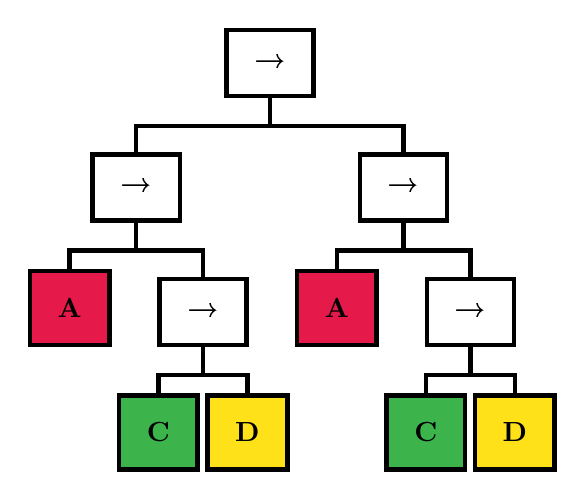
\begin{tikzpicture}

  \tikzstyle{ast} = [%
  align=center,
  draw=black,
  font=\bfseries,
  inner sep=10pt,
  line width=3pt,
  rectangle,
  ultra thick,
  ];

  \tikzset{level distance=45pt};
  \tikzset{edge from parent/.style=
    {
      draw,
      edge from parent path={(\tikzparentnode.south)
        -- +(0,-10pt)
        -| (\tikzchildnode.north)},
      ultra thick,
    }
  }

  \Tree
  [.\node[ast]{→};
    [.\node[ast]{→};
      [.\node[ast,fill=color01]{A}; ]
      [.\node[ast]{→};
        [.\node[ast,fill=color02]{C};]
        [.\node[ast,fill=color03]{D};]
      ]
    ]
    [.\node[ast]{→};
      [.\node[ast,fill=color01]{A}; ]
      [.\node[ast]{→};
        [.\node[ast,fill=color02]{C};]
        [.\node[ast,fill=color03]{D};]
      ]
    ]
  ]

\end{tikzpicture}

\begin{forest}
  for tree={
    align=center,
    draw=black,
    edge={
      ultra thick,
    },
    edge path={
      \noexpand\path[\forestoption{edge}]
      (!u.parent anchor)
      -- +(0,-10pt)
      -| (.child anchor)
      \forestoption{edge label};
    },
    font=\bfseries,
    %inner sep=10pt,
    %line width=2pt,
    minimum width=20pt,
    parent anchor=south,
    rectangle,
    ultra thick,
  }
  [→
    [→
      [A]
      [→ [C] [D]]
    ]
    [→
      [A]
      [→ [C] [D]]
    ]
  ]
\end{forest}

